\documentclass{article}
\usepackage[utf8]{inputenc}
\usepackage[T2A]{fontenc}
\usepackage[russian]{babel}

\usepackage{natbib}
\usepackage{graphicx}
\usepackage{amsmath}
\usepackage{xcolor}
\usepackage{amssymb}
\usepackage{graphicx}
\usepackage[paper=a4paper, margin=2cm, bottom=2cm]{geometry}
\usepackage{pythonhighlight}

\begin{document}
\begin{titlepage}


\newgeometry{margin=1cm}

\centerline{\large \bf МИНИСТЕРСТВО ОБРАЗОВАНИЯ РЕСПУБЛИКИ БЕЛАРУСЬ}
\bigskip
\bigskip
\centerline{\large \bf БЕЛОРУССКИЙ ГОСУДАРСТВЕННЫЙ УНИВЕРСИТЕТ}
\bigskip
\bigskip
\centerline{\large \bf ФАКУЛЬТЕТ ПРИКЛАДНОЙ МАТЕМАТИКИ И ИНФОРМАТИКИ}
\vfill
\centerline{\Large \bf МЕТОДЫ ЧИСЛЕННОГО АНАЛИЗА}
\bigskip
\vfill

\centerline{\Large \bf Лабараторная работа №3}
\bigskip
\centerline{\Large \bf Приближенное вычисление интегралов}
\centerline{\Large \bf с помощью квадратурной формы Гаусса}
\vfill

\hfill
\begin{minipage}{0.25\textwidth}
	{\large{\bf Студент \\ 2 курса 2 группы} \\
		{\it Царик Виталий \\ Александрович }}
\end{minipage}

\vfill
\hfill
\begin{minipage}{0.25\textwidth}
  {\large{\bf Преподаватель} \\
{\it Никифоров Иван \\ Васильевич}}
\end{minipage}
\vfill
\vfill
\centerline{\Large \bf Минск 2019}

\end{titlepage}

\restoregeometry

\section{Условие}
Используя составную двухточечную квадратурную форму Гаусса, посчитать интеграл функции $f(x)$ на отрезке $[a,b]$ с точностью $\varepsilon = 10^{-6}$

\section{Вариант}
\begin{equation}
\label{eq:variant}
f(x) = -\frac{1}{x} + x + x^2, x \in [1, 2]
\end{equation}

\section{Теория}

$\int_{a}^{b}f(x)dx \approx \frac{b-a}{2}(f(\frac{a+b}{2} - \frac{b-a}{2 \sqrt{3}}) + f(\frac{a+b}{2} + \frac{b-a}{2 \sqrt{3}}))$

\section{Исходный код}

\begin{python}
import math
from scipy.integrate import fixed_quad

A = 1
B = 2
EPS = 1e-6
QUAD_INTEGRATION_ORDER = 2


def f(x):
	return -1/x + x + x*x


if __name__ == '__main__':
	diff = math.inf
	prev = fixed_quad(f, A, B, n=QUAD_INTEGRATION_ORDER)[0]
	n = 2

	while diff > EPS:
		total = 0
		h = (B-A)/n
		for i in range(n):
			a = A + h*i
			b = a + h
			total += fixed_quad(f, a, b, n=QUAD_INTEGRATION_ORDER)[0]

		n *= 2
		diff = abs(total - prev)
		prev = total

	print('Approximated value: {}\nNumber of intervals: {}'.format(total, n))

\end{python}

\section{Выходные данные}

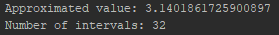
\includegraphics[width=0.7\linewidth]{screenshot001}

\section{Выводы}

Приближение с помощью составной двухточечной квадратурной формы Гаусса являются довольно точным для данной функции даже при относительно небольшом 
количестве отрезков разбиения
\end{document}